\documentclass{article}
\usepackage{graphicx}
\usepackage{amsmath,amsthm,amssymb}
\usepackage[font=small,labelfont=bf]{caption}
\usepackage{tikz}
\usetikzlibrary{calc, angles, quotes, shapes.geometric}
\usepackage{tkz-euclide}
\usepackage[inline]{asymptote}
\usepackage{float}
\usepackage[margin=1in]{geometry}
\usepackage{gensymb}
\usepackage{hyperref}
\hypersetup{
    colorlinks=true,
    linkcolor=blue,
    filecolor=magenta,      
    urlcolor=cyan,
    pdftitle={Overleaf Example},
    pdfpagemode=FullScreen,
    }
\usepackage{fancyhdr}
\pagestyle{fancy}
\fancyhead[R]{Enoch Yu}
\pagenumbering{gobble}
\usepackage{enumitem}
\newtheorem{theorem}{Theorem}[section]
\newtheorem{lemma}[theorem]{Lemma}
\newtheorem*{lemma*}{Lemma}
\newtheorem{sublemma}{Lemma}[section]
\newtheorem{proposition}{Proposition}
\newtheorem{corollary}{Corollary}[theorem]
\newenvironment{solution}{\begin{trivlist}\item[]{\bf Solution}}{\qed \end{trivlist}}
\newcommand{\verteq}{\rotatebox{90}{$\;\;=\;\;$}}
\newcommand*\circled[1]{\tikz[baseline=(char.base)]{
            \node[shape=circle,draw,inner sep=1pt] (char) {#1};}}
\newcommand{\triangled}[1]{\tikz[baseline=(char.base)]{
            \node[shape=regular polygon, regular polygon sides=3, draw, inner sep=0.2pt] (char) {#1};}}

\title{Problem Set 16}
\author{Enoch Yu}
\date{June 2025}

\begin{document}

\section*{2021 AMC 12B Problem 14}
Let $ABCD$ be a rectangle and let $\overline{DM}$ be a segment perpendicular to the plane of $ABCD$. Suppose that $\overline{DM}$ has integer length, and the lengths of $\overline{MA},\overline{MC},$ and $\overline{MB}$ are consecutive odd positive integers (in this order). What is the volume of pyramid $MABCD$?
\\\\
$\textbf{(A) }24\sqrt5 \qquad \textbf{(B) }60 \qquad \textbf{(C) }28\sqrt5\qquad \textbf{(D) }66 \qquad \textbf{(E) }8\sqrt{70}$
\begin{solution}
\\\\
\textbf{Key Word} Pythagorean Theorem
\\\\
First and foremost, the diagram must be drawn.
\begin{center}
    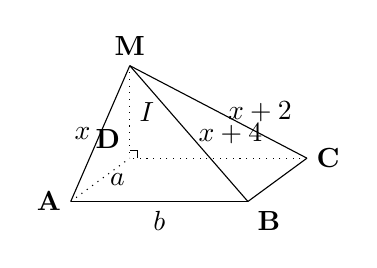
\begin{tikzpicture}[scale=0.5]
        \coordinate (A) at (0,0);
        \coordinate (B) at (4.5,0);
        \coordinate (C) at (6,1.1);
        \coordinate (D) at (1.5,1.1);
        \coordinate (M) at (1.5,3.45);
    
        \draw[dotted] (A) -- (D);
        \draw[dotted] (C) -- (D);
        \draw (A) -- (B);
        \draw (C) -- (B);
    
        \draw (M) -- (A);
        \draw (M) -- (B);
        \draw (M) -- (C);
        \draw[dotted] (M) -- (D);
    
        \draw (1.5, 1.3) -- (1.7, 1.3) -- (1.7, 1.1);
    
        \node[left] at (A) {\textbf{A}};
        \node[below right] at (B) {\textbf{B}};
        \node[right] at (C) {\textbf{C}};
        \node[above left] at (D) {\textbf{D}};
        \node[above] at (M) {\textbf{M}};

        \node[left] at ($(A)!0.5!(M)$) {$x$};
        \node[right] at ($(B)!0.5!(M)$) {$x+4$};
        \node[right] at ($(C)!0.5!(M)$) {$x+2$};
        \node[right] at ($(A)!0.5!(D)$) {$a$};
        \node[below] at ($(A)!0.5!(B)$) {$b$};
        \node[right] at ($(M)!0.5!(D)$) {$I$};
    \end{tikzpicture}
\end{center}
With the diagram, an impulse to utilize Pythagorean theorem is created. Thereby, the shaded right triangles may be used.
\begin{center}
    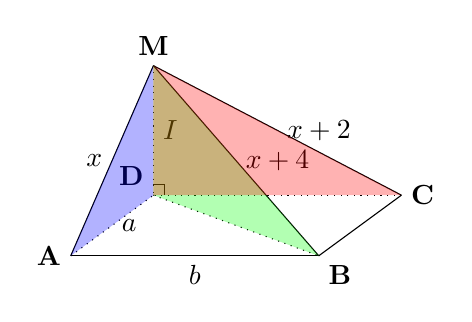
\begin{tikzpicture}[scale=0.7]
        \coordinate (A) at (0,0);
        \coordinate (B) at (4.5,0);
        \coordinate (C) at (6,1.1);
        \coordinate (D) at (1.5,1.1);
        \coordinate (M) at (1.5,3.45);
    
        \draw[dotted] (A) -- (D);
        \draw[dotted] (C) -- (D);
        \draw (A) -- (B);
        \draw (C) -- (B);
        \draw[dotted] (D) -- (B);
    
        \draw (M) -- (A);
        \draw (M) -- (B);
        \draw (M) -- (C);
        \draw[dotted] (M) -- (D);
    
        \draw (1.5, 1.3) -- (1.7, 1.3) -- (1.7, 1.1);
    
        \node[left] at (A) {\textbf{A}};
        \node[below right] at (B) {\textbf{B}};
        \node[right] at (C) {\textbf{C}};
        \node[above left] at (D) {\textbf{D}};
        \node[above] at (M) {\textbf{M}};

        \node[left] at ($(A)!0.5!(M)$) {$x$};
        \node[right] at ($(B)!0.5!(M)$) {$x+4$};
        \node[right] at ($(C)!0.5!(M)$) {$x+2$};
        \node[right] at ($(A)!0.5!(D)$) {$a$};
        \node[below] at ($(A)!0.5!(B)$) {$b$};
        \node[right] at ($(M)!0.5!(D)$) {$I$};

        \fill[blue, opacity=0.3] (A) -- (D) -- (M);
        \fill[green, opacity=0.3] (B) -- (D) -- (M);
        \fill[red, opacity=0.3] (C) -- (D) -- (M);
    \end{tikzpicture}
\end{center}
The following equations could be obtained from Pythagorean Theorem.
\begin{align*}
    I^2+a^2&=x^2 \\
    I^2+b^2&=(x+2)^2 \\
    I^2+a^2+b^2&=(x+4)^2 \\
\end{align*}
Because $x$ and $I$ are integers, writing an equation in terms of only $x$ and $I$ may be beneficial for trial and error.
\begin{align*}
    x^2+(x+2)^2&=(x+4)^2+I^2 \\
    2x^2+4x+4&=x^2+8x+16+I^2 \\
    x^2-4x-12&=I^2 \\
    (x-6)(x+2)&=I^2
\end{align*}
$x=7$ seems valid since $I=3$ when $x=7$. Therefore, when $x=7$, $a=2\sqrt{10}$ and $b=6\sqrt{2}$. We could double check that $40+72+9=11^2$. Thereby,
\[
\frac{a\cdot b\cdot I}{3}=\frac{2\sqrt{10}\cdot6\sqrt{2}\cdot3}{3}=\boxed{\textbf{(A) }24\sqrt5}.
\]
\end{solution}
Uploaded a \href{https://artofproblemsolving.com/wiki/index.php/2021_AMC_12B_Problems/Problem_14#Solution_3}{new solution} in AOPS!! \\
\includegraphics[scale=0.02]{Screenshot 2025-06-04 at 6.13.23 PM.png}

\newpage
\section*{2021 AMC 12B Problem 21}
Problem 21
Let $S$ be the sum of all positive real numbers $x$ for which\[x^{2^{\sqrt2}}=\sqrt2^{2^x}.\]Which of the following statements is true?
\\\\
$\textbf{(A) }S<\sqrt2 \qquad \textbf{(B) }S=\sqrt2 \qquad \textbf{(C) }\sqrt2<S<2\qquad \textbf{(D) }2\le S<6 \qquad \textbf{(E) }S\ge 6$
\begin{solution}
\\\\
\textbf{Key Word} Approximation
\\\\
While utilizing $\log$ may seem conventional, graphing may also be used. Notice that $x^{2^{\sqrt2}}$ is a U-shaped, differentiable curve. Moreover, $\sqrt2^{2^x}$ is an exponentially increasing function. Furthermore, we could notice that the two graphs meet at $x=\sqrt{2}$.
\[
\begin{array}{c|c|c|c}
    x & x^{2^{\sqrt2}} & \sqrt2^{2^x} & \text{Comparison} \\
    \hline
    0 & 0 & \sqrt{2} & x^{2^{\sqrt2}} < \sqrt2^{2^x} \\
    1 & 2<2^{\sqrt{2}}<4 & 2 & x^{2^{\sqrt2}} < \sqrt2^{2^x} \\
    \sqrt{2} & {\sqrt{2}}^{2^{\sqrt2}} & {\sqrt{2}}^{2^{\sqrt2}} & x^{2^{\sqrt2}} = \sqrt2^{2^x} \\
    2 & 4<2^{2^{\sqrt2}}<16 & 4 & x^{2^{\sqrt2}} > \sqrt2^{2^x} \\
    3 & 9<3^{2^{\sqrt2}}<81 & 16 & NA \\
    4 & 16<4^{2^{\sqrt2}}<256 & 256 & x^{2^{\sqrt2}} < \sqrt2^{2^x} \\
\end{array}
\]
Because the $x^2<x^{2^{\sqrt2}}<x^4$ and $\sqrt2^{2^x}$ is an exponentially increasing function, $x^{2^{\sqrt2}}$ can never meet or catch up $\sqrt2^{2^x}$ from $x\ge4$. In another words, only two intersections, or the roots of the equation, exists. The roots are $\sqrt{2}$ and a constant in the interval $2<r_2<4$. Let $S=\sqrt{2}+r_2$. It is evident that the possible range for $S$ is $\boxed{\textbf{(D) }2\le S<6}$.
\end{solution}
Uploaded a \href{https://artofproblemsolving.com/wiki/index.php/2021_AMC_12B_Problems/Problem_21#Solution_3_.28No_Logarithm.29}{new solution} in AOPS!! \\
\includegraphics[scale=0.45]{Screenshot 2025-06-04 at 7.15.47 PM.png}

\newpage
\section*{2021 AMC 12B Problem 24}
Let $ABCD$ be a parallelogram with area $15$. Points $P$ and $Q$ are the projections of $A$ and $C,$ respectively, onto the line $BD;$ and points $R$ and $S$ are the projections of $B$ and $D,$ respectively, onto the line $AC.$ See the figure, which also shows the relative locations of these points.
\begin{center}
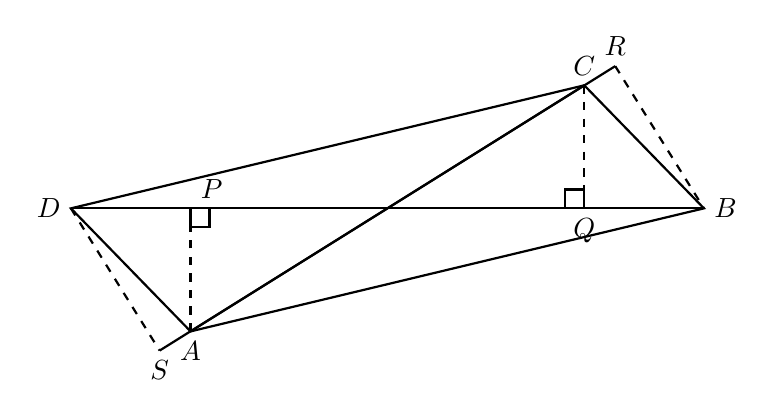
\begin{tikzpicture}[scale=1.2, 
                    thick,
                    dot/.style={fill, circle, inner sep=1.5pt},
                    right angle/.style={draw,–, shift={(#1)}, rotate=##2}
                    ]
    \def\Ax{-2.0833333333}   \def\Ay{-1.3020833333}
    \def\Bx{ 3.3500000000}   \def\By{ 0.0000000000}
    \def\Cx{ 2.0833333333}   \def\Cy{ 1.3020833333}
    \def\Dx{-3.3500000000}   \def\Dy{ 0.0000000000}
    
    \def\Px{-2.0833333333}   \def\Py{ 0.0000000000}
    \def\Qx{ 2.0833333333}   \def\Qy{ 0.0000000000}
    \def\Rx{ 2.4109375000}   \def\Ry{ 1.5052083333}
    \def\Sx{-2.4109375000}   \def\Sy{-1.5052083333}
    
    \coordinate (A) at (\Ax,\Ay);
    \coordinate (B) at (\Bx,\By);
    \coordinate (C) at (\Cx,\Cy);
    \coordinate (D) at (\Dx,\Dy);
    \coordinate (P) at (\Px,\Py);
    \coordinate (Q) at (\Qx,\Qy);
    \coordinate (R) at (\Rx,\Ry);
    \coordinate (S) at (\Sx,\Sy);
    
    \draw (A)--(B)--(C)--(D)--cycle;
    \draw (A)--(C);
    \draw (B)--(D);
    
    \draw[dashed] (A)--(P);
    \draw[dashed] (C)--(Q);
    \draw[dashed] (D)--(S) (R)--(B);
    
    \draw (R)--(S);
    
    \tkzMarkRightAngle[size=.2](A,P,Q);
    \tkzMarkRightAngle[size=.2](C,Q,D);
    
    \node[below] at (A) {$A$};
    \node[right] at (B) {$B$};
    \node[above] at (C) {$C$};
    \node[left] at (D) {$D$};
    \node[above right] at (P) {$P$};
    \node[below] at (Q) {$Q$};
    \node[above] at (R) {$R$};
    \node[below] at (S) {$S$};
\end{tikzpicture}
\end{center}
Suppose $PQ=6$ and $RS=8,$ and let $d$ denote the length of $\overline{BD},$ the longer diagonal of $ABCD.$ Then $d^2$ can be written in the form $m+n\sqrt p,$ where $m,n,$ and $p$ are positive integers and $p$ is not divisible by the square of any prime. What is $m+n+p?$
\\\\
$\textbf{(A) }81 \qquad \textbf{(B) }89 \qquad \textbf{(C) }97\qquad \textbf{(D) }105 \qquad \textbf{(E) }113$
\begin{solution}
\\\\
\textbf{Key Word} Pythagorean Theorem
\\\\
First and foremost, the condition given in the problem could be represented. Moreover, let $QB=x$ and $CQ=h$ for convenience.
\begin{center}
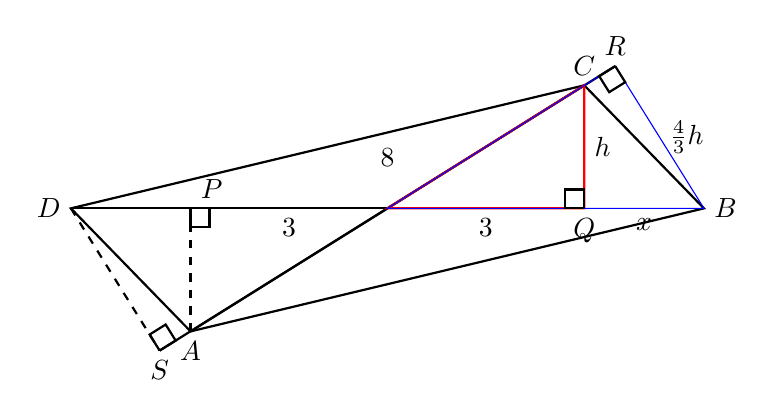
\begin{tikzpicture}[scale=1.2, 
                    thick,
                    dot/.style={fill, circle, inner sep=1.5pt},
                    right angle/.style={draw,–, shift={(#1)}, rotate=##2}
                    ]
    \def\Ax{-2.0833333333}   \def\Ay{-1.3020833333}
    \def\Bx{ 3.3500000000}   \def\By{ 0.0000000000}
    \def\Cx{ 2.0833333333}   \def\Cy{ 1.3020833333}
    \def\Dx{-3.3500000000}   \def\Dy{ 0.0000000000}
    
    \def\Px{-2.0833333333}   \def\Py{ 0.0000000000}
    \def\Qx{ 2.0833333333}   \def\Qy{ 0.0000000000}
    \def\Rx{ 2.4109375000}   \def\Ry{ 1.5052083333}
    \def\Sx{-2.4109375000}   \def\Sy{-1.5052083333}
    
    \coordinate (A) at (\Ax,\Ay);
    \coordinate (B) at (\Bx,\By);
    \coordinate (C) at (\Cx,\Cy);
    \coordinate (D) at (\Dx,\Dy);
    \coordinate (P) at (\Px,\Py);
    \coordinate (Q) at (\Qx,\Qy);
    \coordinate (R) at (\Rx,\Ry);
    \coordinate (S) at (\Sx,\Sy);
    \coordinate (O) at (0,0);
    
    \draw (A)--(B)--(C)--(D)--cycle;
    \draw (A)--(C);
    \draw (D) -- (O);
    
    \draw[dashed] (A)--(P);
    \draw[dashed] (D)--(S);
    
    \draw (R)--(S);

    \draw[color=red, thick] (O) -- (C) -- (Q) -- cycle;
    \draw[color=blue, thin] (O) -- (B) -- (R) -- cycle;
    
    \tkzMarkRightAngle[size=.2](A,P,Q);
    \tkzMarkRightAngle[size=.2](C,Q,D);
    \tkzMarkRightAngle[size=.2](D,S,R);
    \tkzMarkRightAngle[size=.2](B,R,S);
    
    \node[below] at (A) {$A$};
    \node[right] at (B) {$B$};
    \node[above] at (C) {$C$};
    \node[left] at (D) {$D$};
    \node[above right] at (P) {$P$};
    \node[below] at (Q) {$Q$};
    \node[above] at (R) {$R$};
    \node[below] at (S) {$S$};

    \node[below] at ($(P)!0.5!(O)$) {$3$};
    \node[below] at ($(O)!0.5!(Q)$) {$3$};
    \node[below] at ($(Q)!0.5!(B)$) {$x$};
    \node[right] at ($(C)!0.5!(Q)$) {$h$};
    \node[right] at ($(R)!0.5!(B)$) {$\frac{4}{3}h$};
    \node[above=.4] at ($(R)!0.5!(S)$) {$8$};
\end{tikzpicture}
\end{center}
Using the property of a parallelogram, it could be inferred that $\frac{h(3+x)}{2}=\frac{15}{4}$. Moreover, Pythagorean Theorem manifests that $\left(\frac{4}{3}h\right)^2+4^2=(3+x)^2$.
\begin{align*}
    3+x&=\frac{15}{2h} \\
    \left(\frac{4}{3}h\right)^2+4^2&=\left(\frac{15}{2h}\right)^2 \\
    \frac{16h^2}{9}+16&=\frac{225}{4h^2} \\
    64h^4+576h^2-2025&=0 \\
    h^2&\Rightarrow\frac{9\sqrt{41}-36}{8}
\end{align*}
\begin{align*}
    \left(\frac{4}{3}h\right)^2+4^2&=(3+x)^2 \\
    \frac{16}{9}\cdot\frac{9\sqrt{41}-36}{8}+4^2&=(3+x)^2 \\
    2\sqrt{41}-8+16&=(3+x)^2 \\
    (3+x)^2&=8+2\sqrt{41} \\
    d^2=4(3+x)^2&=32+8\sqrt{41}
\end{align*}
Thus, $32+8+41=\boxed{\textbf{(A) }81}$.
\end{solution}
Uploaded a \href{https://artofproblemsolving.com/wiki/index.php/2021_AMC_12B_Problems/Problem_24#Solution_8}{new solution} in AOPS!! \\
\includegraphics[scale=0.5]{Screenshot 2025-06-05 at 4.38.19 PM.png}

\newpage
\section*{2021 AMC 12B Problem 19}
Two fair dice, each with at least $6$ faces are rolled. On each face of each die is printed a distinct integer from $1$ to the number of faces on that die, inclusive. The probability of rolling a sum of $7$ is $\frac34$ of the probability of rolling a sum of $10,$ and the probability of rolling a sum of $12$ is $\frac{1}{12}$. What is the least possible number of faces on the two dice combined?
\\\\
$\textbf{(A) }16 \qquad \textbf{(B) }17 \qquad \textbf{(C) }18\qquad \textbf{(D) }19 \qquad \textbf{(E) }20$
\begin{solution}
\\\\
\textbf{Key Word} Logic, Trial and Error
\\\\
Notice that
\begin{align*}
    7&=1+6 \\
    &\ \ \ \ \ \ \ \ \ \vdots \\
    &=6+1
\end{align*}
are the only cases that could possibly form 7. In another words, regardless of the number of faces for each dice, 6 is the number of cases that could form a rolling sum of 7.
\\\\
Because the value of the total combination for both are the same, we could infer that the number of cases of having a rolling sum of 10 is $\frac{4}{3}\cdot6=8$. With the number 8, we could also deduce that one dice has 8 sides and the other has at least 9 sides. Thence trial and error could be utilized.
\\\\
Since 9 is the next smallest number, the case could be tested.
\begin{align*}
    12&=3+9 \\
    &=4+8 \\
    &\ \ \ \ \ \ \ \ \ \vdots \\
    &=8+4
\end{align*}
$\frac{6}{8\cdot9}=\frac{1}{12}$ is also true. Therefore, $8+9=\boxed{\textbf{(B) }17}$
\end{solution}
Uploaded a 
\href{https://artofproblemsolving.com/wiki/index.php/2021_AMC_12B_Problems/Problem_19#Solution_3_.28Logic.29}{new solution} in AOPS!! \\
\includegraphics[scale=0.3]{Screenshot 2025-06-05 at 5.26.59 PM.png}

\end{document}
